Using the LEV detection and tracking procedure developed in Section \ref{sec:LEV_detect_track}, a quantitative comparison of the LEV is presented in this section. 
Figure \ref{fig:zonal_LEV_radius_Re200k} shows the LEV core radius ($r_c$) for different meshes at multiple phases.

M0\_nz50 mesh shows the largest radius among all the meshes, and fails to capture the trend that the other finer meshes show.
Mza1\_nz50 mesh follows a similar trend as Mza2\_nz50 mesh.
Mza2\_nz50 shows the lowest radius among all the meshes, which is expected as mesh resolution is the highest in this mesh, and as a result, a less diffused LEV is obtained.

\begin{figure}[H]
	\centering
	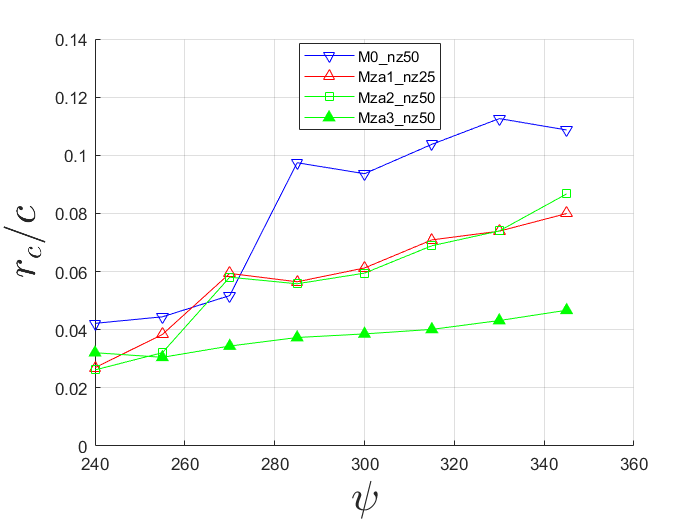
\includegraphics[width=0.7\textwidth]{figures/zonal_adapt_results/LEV_Re200k/LEV_radius_vp}
	\caption{ Adaptive LES at $Re = 200,000$: LEV size}
	\label{fig:zonal_LEV_radius_Re200k}
\end{figure}

Figure \ref{fig:zonal_LEV_location_Re200k} shows the location of the center of the LEV for different phases after it is ejected from the airfoil surface. 
Note that the LEV is ejected closer to the leading edge as compared to the lower Reynolds number case of $Re=40,000$ (for the same advance ratio).
M0\_nz50 mesh shows differences for LEV path from Mza1\_nz50 and Mza2\_nz50 meshes. LEV shows a similar path for Mza1\_nz50 and Mza2\_nz50 meshes.

\begin{figure}[H]
	\centering
	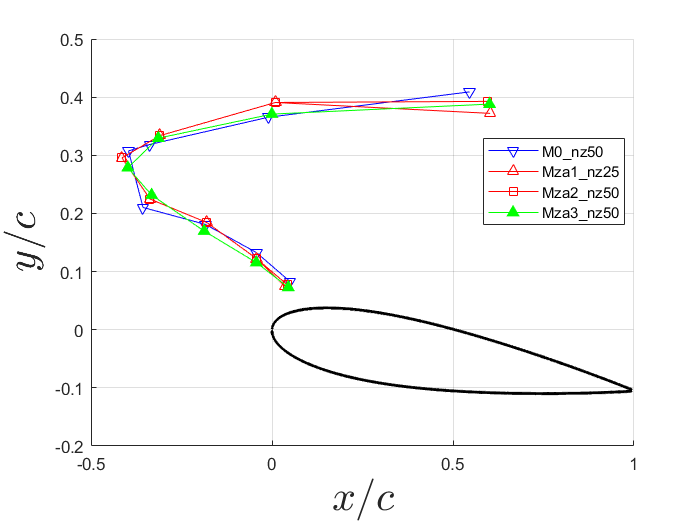
\includegraphics[width=0.75\textwidth]{figures/zonal_adapt_results/LEV_Re200k/LEV_location_Re200k}
	\caption{ Adaptive LES at $Re = 200,000$: LEV position}
	\label{fig:zonal_LEV_location_Re200k}
\end{figure}

Figure \ref{fig:zonal_utheta_LEV_Re200k} shows the tangential/azimuthal velocity ($u_{\theta}$) profiles for the LEV from different meshes at 3 phases of $\psi = 255^\circ$,  $\psi = 270^\circ$ and  $\psi = 300^\circ$. 
Recall that the tangential velocity is computed along multiple radial lines passing through the LEV center, and the mean tangential velocity over these radial lines is shown in Figure \ref{fig:zonal_utheta_LEV}, along with a 95\% confidence interval due to multiple radial lines.
The radial distance from the center of the LEV, $r$, is normalized by the LEV core radius $r_c$ of the finest mesh (Mza2\_nz50 mesh in this case) at that particular phase.

Tangential velocity at the phases shown differs for all the meshes, with M0\_nz50 predicting the lowest tangential velocity, and Mza2\_nz50 predicting the highest.
Note that the confidence interval bounds for these are significantly smaller than for the lower Reynolds number case of $Re=40,000$ at all phases shown here, indicating that the LEV is azimuthally more symmetric at $Re=200,000$ than at $Re=40,000$.

\begin{figure}[H]
	\centering
	\begin{subfigure}[b]{0.475\textwidth}
		\centering
		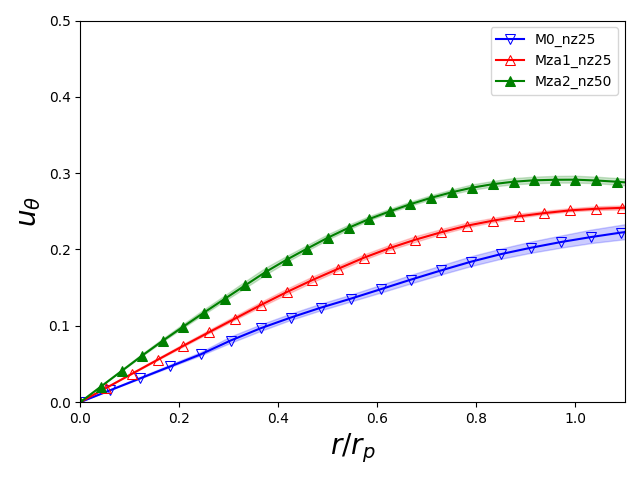
\includegraphics[width=1\textwidth]{figures/zonal_adapt_results/LEV_Re200k/u_theta/phase_255.png}
		\caption{ $u_\theta$ at $\psi$ = $255^\circ$}
		\label{fig:zonal_utheta_255_Re200k}
	\end{subfigure}
	\begin{subfigure}[b]{0.475\textwidth}
		\centering
		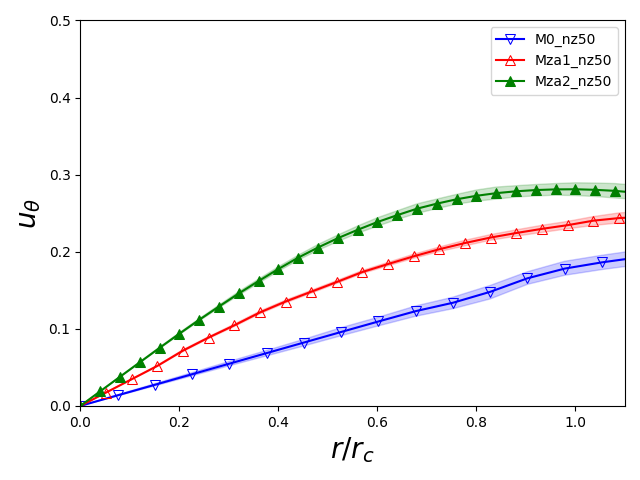
\includegraphics[width=1\textwidth]{figures/zonal_adapt_results/LEV_Re200k/u_theta/phase_270.png}
		\caption{ $u_\theta$ at $\psi$ = $270^\circ$}
		\label{fig:zonal_utheta_270_Re200k}
	\end{subfigure}
	\begin{subfigure}[b]{0.475\textwidth}
		\centering
		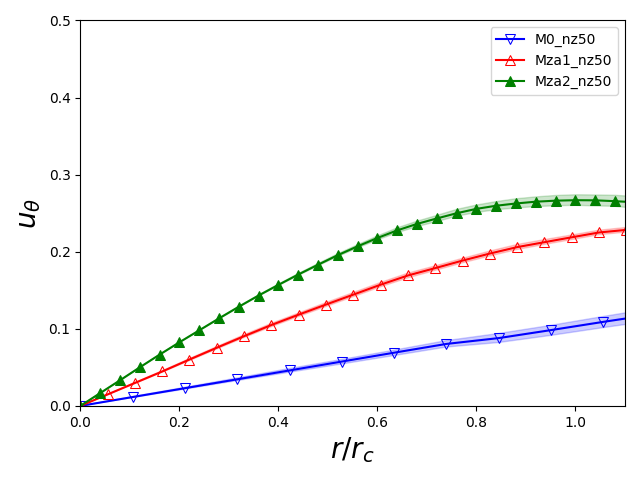
\includegraphics[width=1\textwidth]{figures/zonal_adapt_results/LEV_Re200k/u_theta/phase_300.png}
		\caption{ $u_\theta$ at $\psi$ = $300^\circ$}
		\label{fig:zonal_utheta_300_Re200k}
	\end{subfigure}
	\caption{Adaptive LES at $Re = 200,000$: LEV tangential velocity profile (including 95\% confidence interval)}
	\label{fig:zonal_utheta_LEV_Re200k}
\end{figure}

\subsubsection{Summary}
In summary, a thorough quantitative comparison of relevant quantities, such as spanwise vorticity, $C_p$ and LEV evolution and quantification, is performed for a series of adapted meshes. Similar trends are observed in this case at $Re=200,000$ like the previous case at $Re=40,000$. Mza3 mesh is needed to fully demonstrate mesh convergence for this case.